\chapter{Oracle Aplication Express (APEX) }

\section{Pengenalan Oracle APEX}
Oracle Aplication Express\cite{OracleApex}, adalah aplikasi yang digunakan untuk membangun database yang dikembangkan oleh Oracle atau biasa disebut juga HTML-DB (sementara ini sampai versi terbaru masih dedicated untuk Oracle DB. Oracle APEX Adalah sebuah wadah dan sarana untuk membuat aplikasi yang menggunakan database Oracle Itu sendirMengekspor aplikasi dari Application Express sangat mudah dan menghasilkan file skrip yang dapat dibaca dengan ekstensi .SQL. Script SQL ini dapat dijalankan di lingkungan Oracle Application Express mana pun yang merupakan rilis yang sama atau lebih tinggi dari Application Express dari tempat itu diekspor. Misalnya, aplikasi yang diekspor dari Application Express 4.0 dapat diimpor ke lingkungan yang menjalankan Application Express 4.0, 4.1, atau 4.2. Namun, aplikasi yang diekspor dari Application Express 4.2 tidak dapat diimpor ke lingkungan yang menjalankan Application Express 4.1 atau yang lebih lama. Ekspor aplikasi mencakup definisi aplikasi, objek pendukung, dan komponen bersama, termasuk plug-in. Namun, ekspor tidak termasuk gambar, file CSS, file JavaScript, dll. Yang harus dikelola secara independen. Selain itu, Application Express memungkinkan pengguna untuk merancang, mengembangkan, dan menggunakan aplikasi berbasis database yang baik dan responsif. Hanya menggunakan browser web, pengguna dapat mengembangkan dan menggunakan aplikasi profesional yang cepat dan aman untuk perangkat apa pun.

\section{Fitur-Fitur Pada Oracle Apex}
Berikut adalah fitur-fitur yang terdapat di aplikasi Oracle Experes :

\begin{enumerate}

\item[1]Application Express engine membantu kita untuk membuat aplikasi secara real time dari data yang sudah disimpan di dalam table database. Ketika anda membuat atau mengembangkan sebuah aplikasi, Oracle Application Express membuat atau memodifikasi metadata yang disimpan dalam table database. Pada saat aplikasi dijalankan, Application Express engine kemudian akan membaca metadata dan menampilkan aplikasi.

\item[2]Drag and Drop file XLS, CSV, XML, atau JSON.
Jadi fitur bisa pengguna gunakan untuk mengembangkan aplikasi yang ingin dibuat dengan oracle apex dengan cara drag and drop file berupa XLS, CSV, XML, atau JSON.
    

\item[3]Membuat tabel dalam Autonomous Database. Oracle Autonomous Database mengotomatiskan semua manajemen database, infrastruktur, pemantauan, dan tuning. Hal ini dapat mengurangi biaya admin, meskipun admin masih akan diperlukan untuk tugas-tugas seperti mengelola bagaimana aplikasi terhubung ke gudang data dan bagaimana pengembang menggunakan fitur dan fungsi dalam basis data.


\item[4]Upload data into a new table. Fitur ini memungkinkan pengguna untuk mengunggah data ke table pada database yang sudah di buat di aplikasi apex.

\item[5]Create App based on new table. tidak hanya dapat menggugah data ataupun drag and drop file dari luar, dengan membuat table baru pada apex oracle, pengguna bisa membuat aplikasi berdasarkan tabel baru yang sudah dibuat oleh pengguna  


\end{enumerate}

\section{Tahapan Pembuatan Aplikasi Oracle Apex}
Langkah pertama yang harus dilakukan adalah membuka website https://apex.oracle.com, disini kita akan mendapatkan akses untuk memasuki Oracle Apllication Express, pastikan email yang dimasukkan valid untuk membuat Workspace, berikut adalah langkah langkah pembuatan Aplikasi pada Oracle APEX :

\begin{enumerate}
    \begin{figure}[!htbp]
    \item[1.] Sebelum kita membuat pastikan kalian sudah membuat workspace, dan kita lngsung ke langkah yang pertama setelah kita membuat workspace.
        \begin{center}
        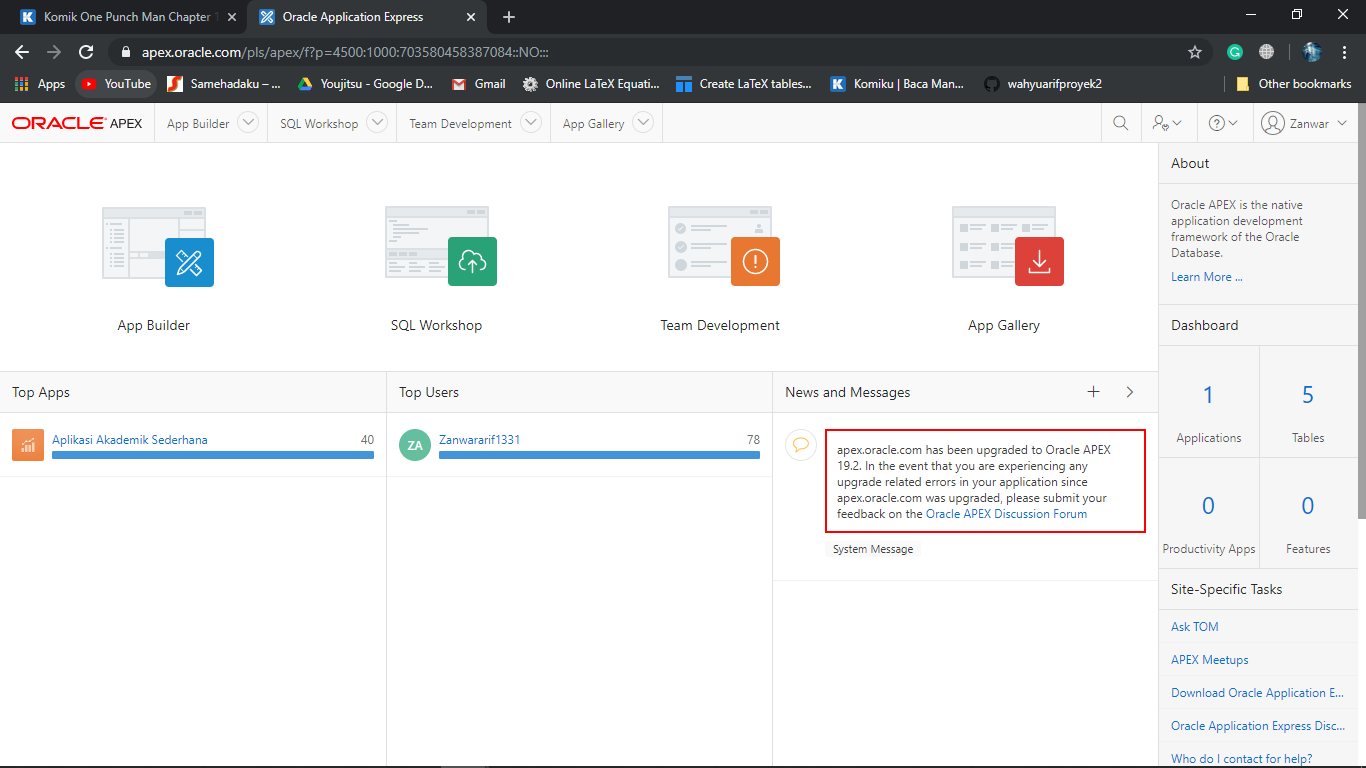
\includegraphics[scale=0.3]{figures/Screenshot(116).png}
        \caption{\textit{Home Oracle Application Express.}}
        \end{center}   
    \end{figure}
    
    \begin{figure}[!htbp]
    \item[2.] Pilih create pada menu aplikasi builder, kemudian kita akan menggunakan cara upload data yang sudah dari file excel.
        \begin{center}
        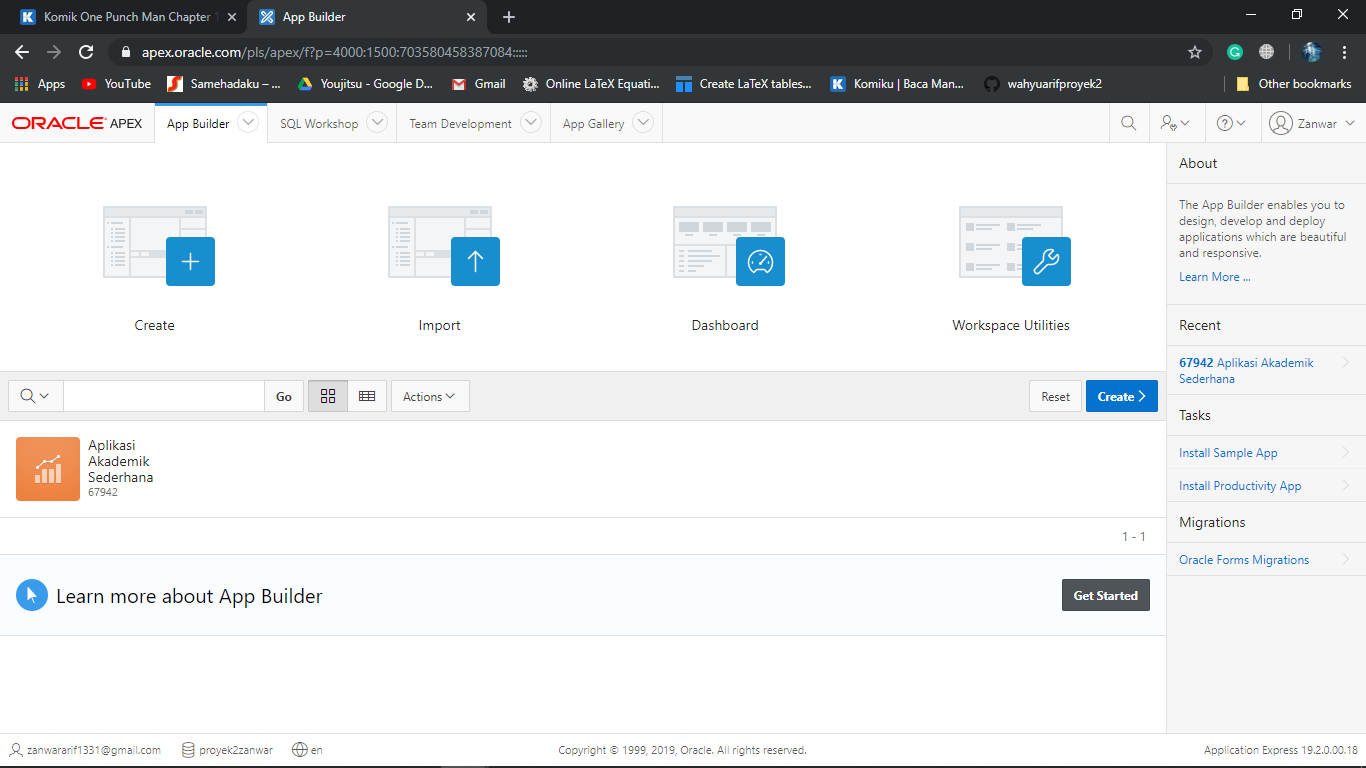
\includegraphics[scale=0.3]{figures/Screenshot(117).png}
        \caption{\textit{Create Application.}}
        \end{center}   
    \end{figure}

    \begin{figure}[!htbp]
    \item[3.] Kemudian pilih file yang akan diupload, tapi ingat filenya harus dengan ekstensi CSV,XLS,TXT,XML, dan JSON. Tapi disini kita mengupload file dengan ekstensi XLS.
        \begin{center}
        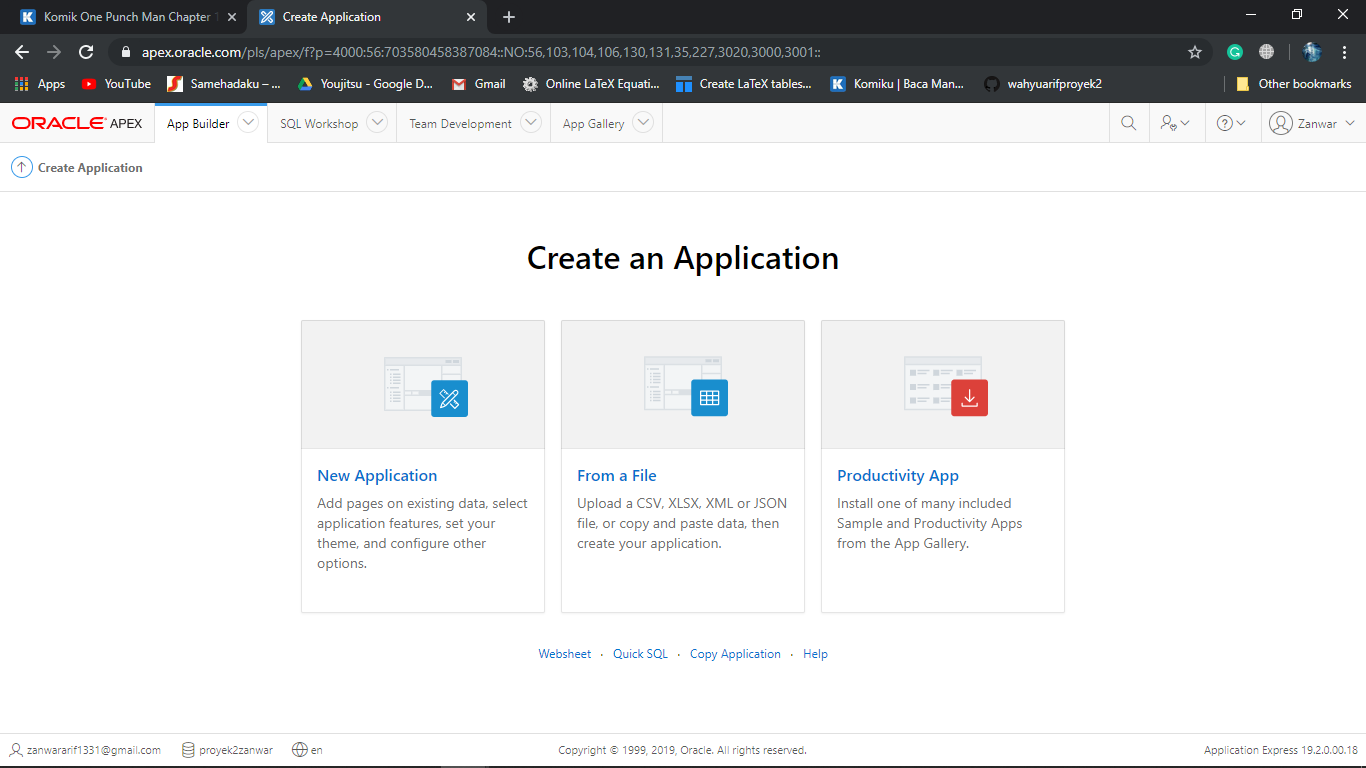
\includegraphics[scale=0.3]{figures/Screenshot(118).png}
        \caption{\textit{Choose File.}}
        \end{center}   
    \end{figure}
    
    \begin{figure}[!htbp]
    \item[4.] Setelah memilih file yang diupload, kita harus ememberikan nama tabel dari file yang kita upload.
    \begin{center}
    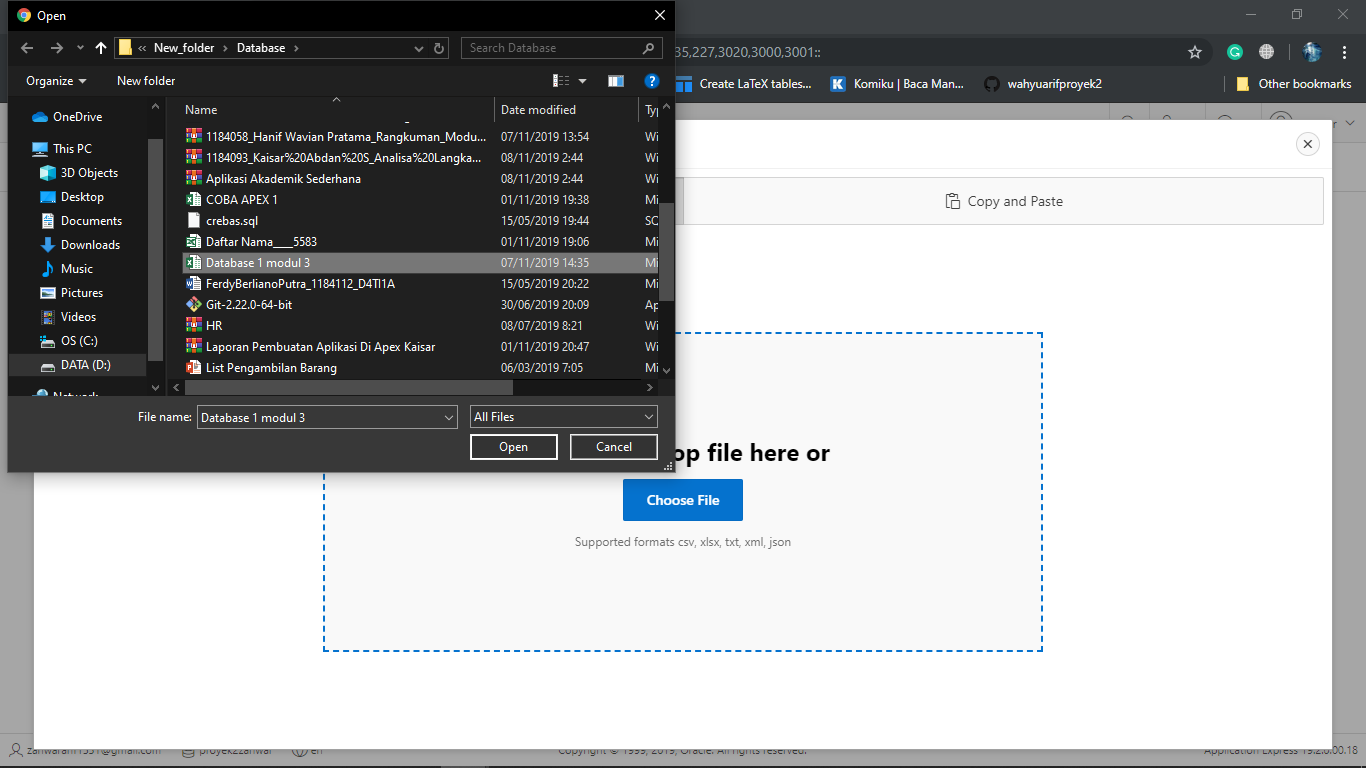
\includegraphics[scale=0.3]{figures/Screenshot(119).png}
    \caption{\textit{Load Data.}}
    \end{center}   
    \end{figure}
    
    \begin{figure}[!htbp]
    \item[5.] Selanjutnya karena kita menggunakan excel, jadi kita harus mengupload table berdasarkan sheetnya, sesuaikan dengan nama tabel.
    \begin{center}
    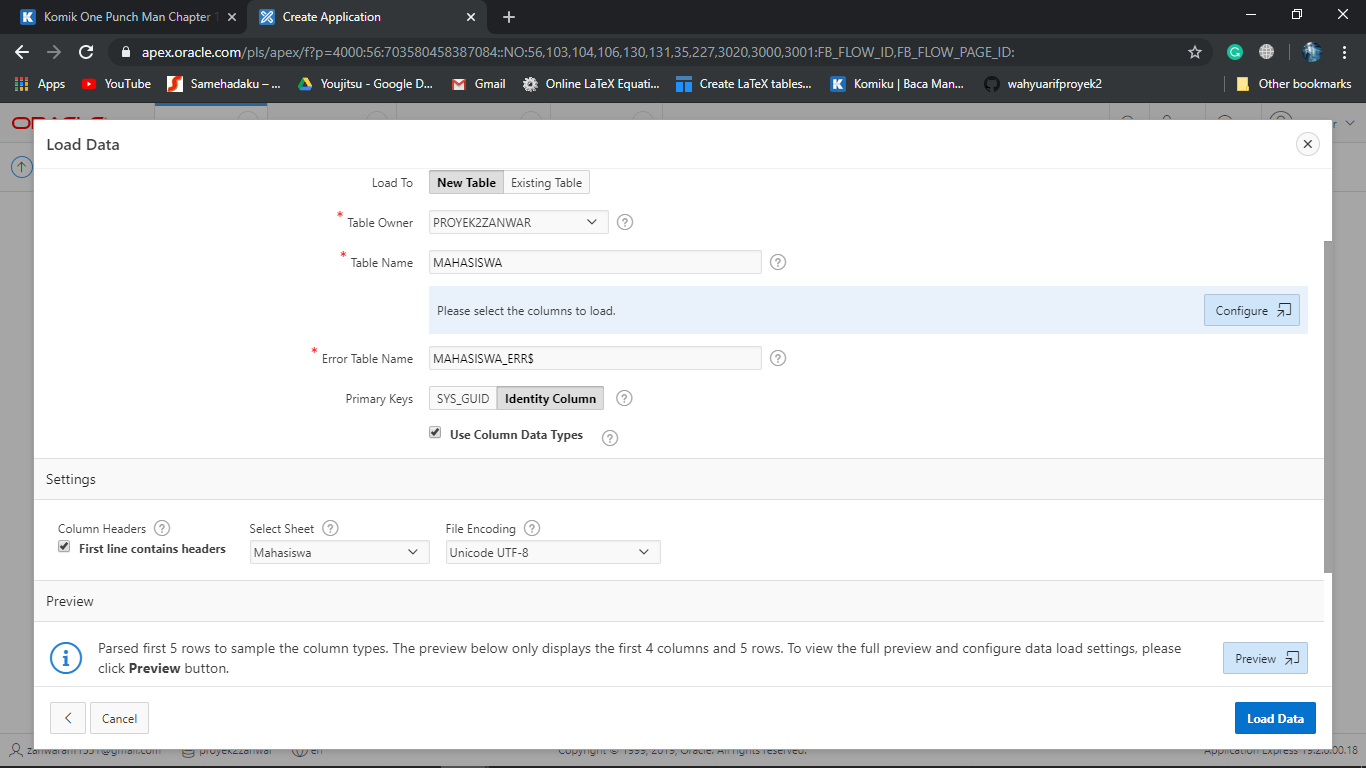
\includegraphics[scale=0.3]{figures/Screenshot(120).png}
    \caption{\textit{Configure Table.}}
    \end{center}   
    \end{figure}
    
    \begin{figure}[!htbp]
    \item[6.] Berikut bentuk tampilan tabel yang sudah kita upload.
    \begin{center}
    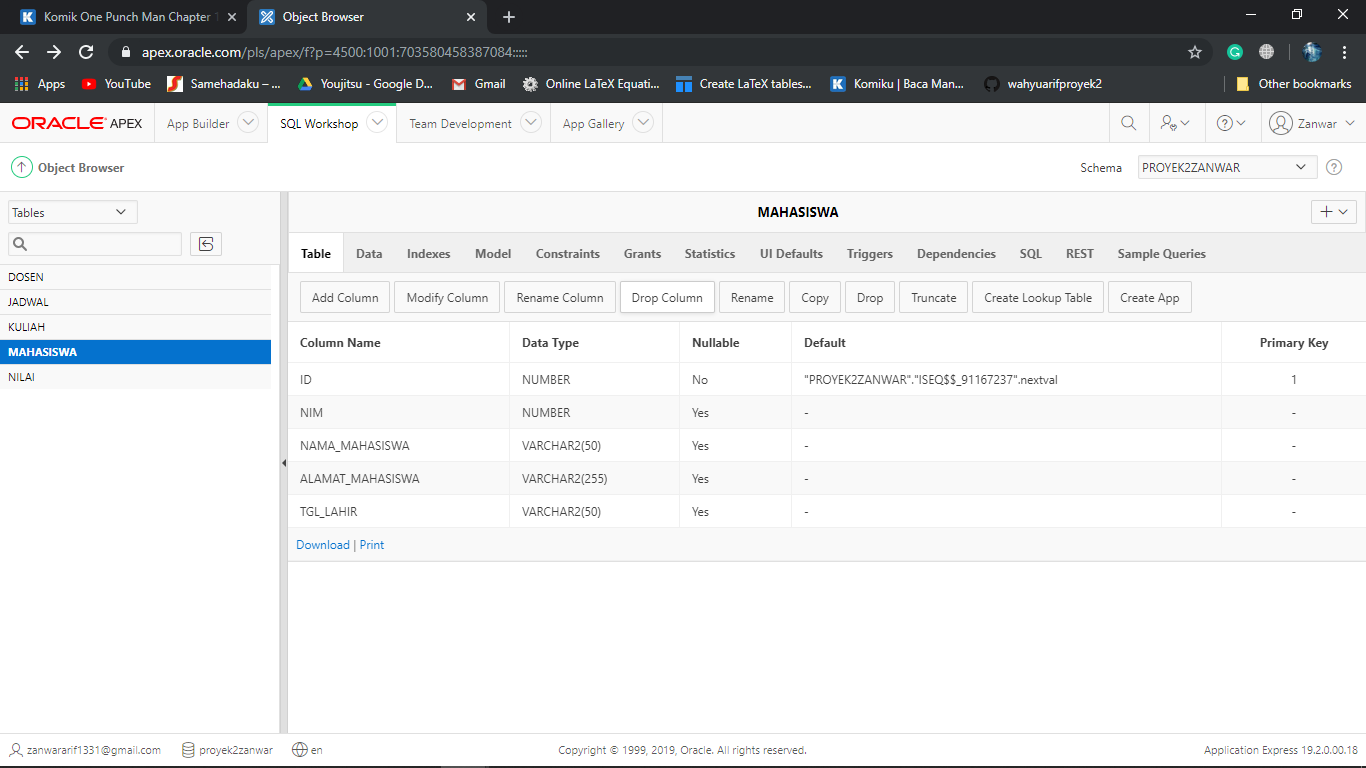
\includegraphics[scale=0.3]{figures/Screenshot(122).png}
    \caption{\textit{Table.}}
    \end{center}   
    \end{figure}
    
    \begin{figure}[!htbp]
    \item[7.] Setelah selesai upload smua Tabel dari setiap Sheet excel yang dibuat, akan tercipta attribut baru yaitu ID sebagai Primary Key. Karena tabel yg kita upload belum memiliki Primary key. Dengan cara Klik Drop Column.
    \begin{center}
    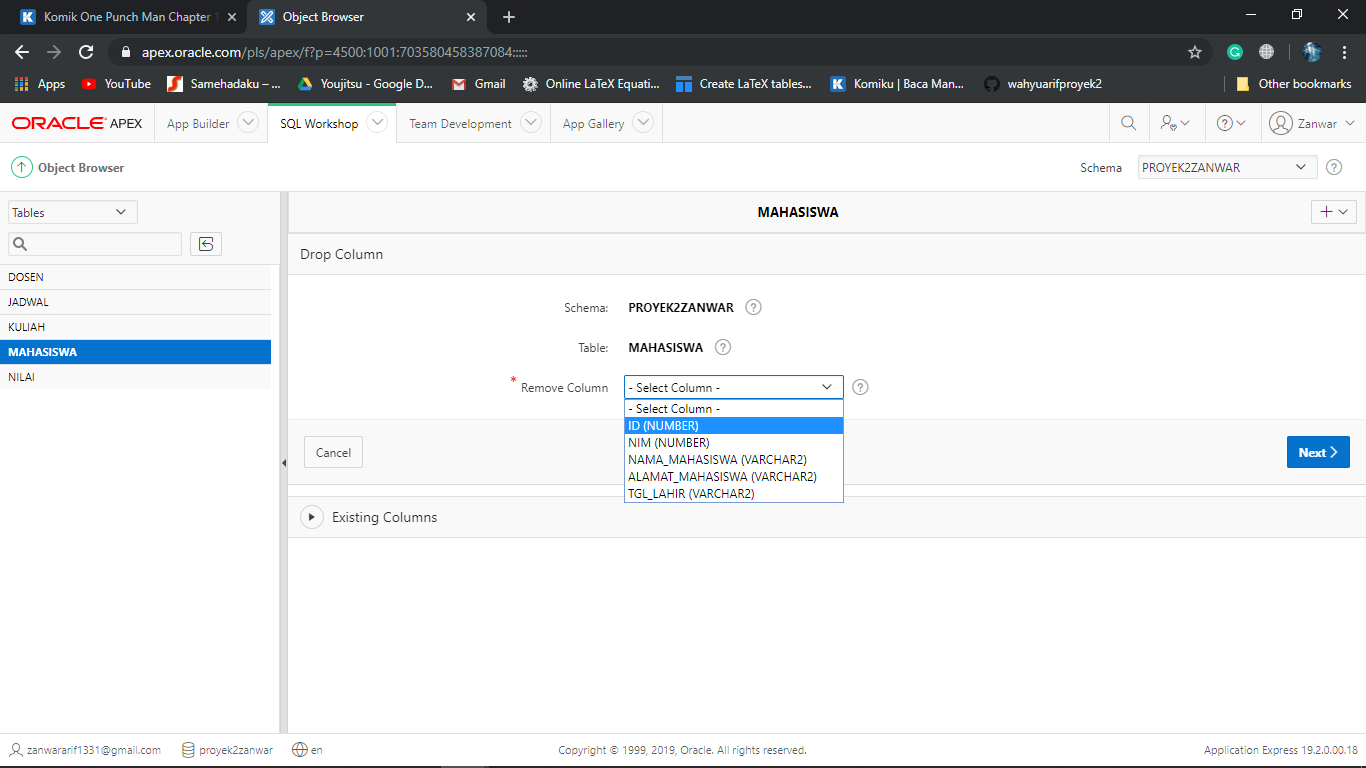
\includegraphics[scale=0.3]{figures/Screenshot(123).png}
    \caption{\textit{Drop ID.}}
    \end{center}   
    \end{figure}
    
    \begin{figure}[!htbp]
    \item[8.] Nah Hapus semua attribut ID di setiap table yaa.
    \begin{center}
    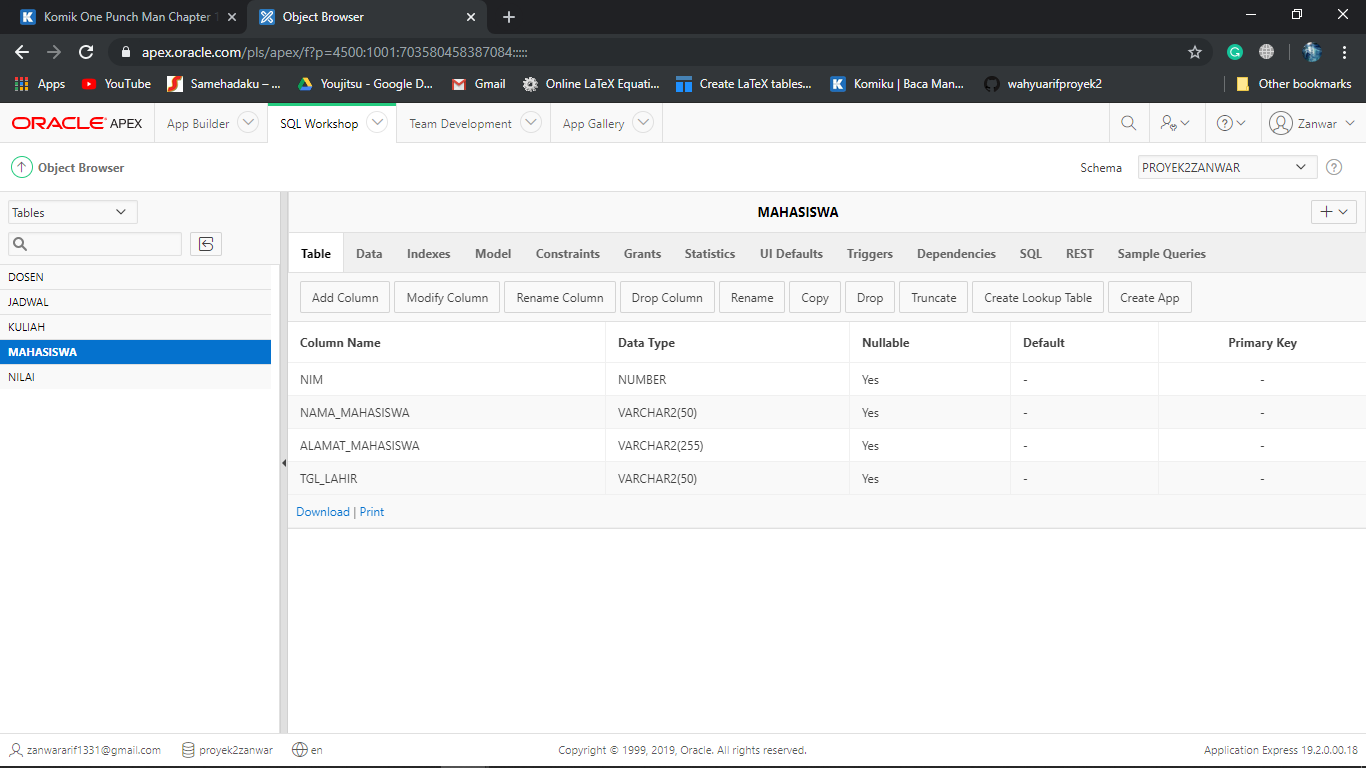
\includegraphics[scale=0.3]{figures/Screenshot(124).png}
    \caption{\textit{No ID.}}
    \end{center}   
    \end{figure}
    
    \begin{figure}[!htbp]
    \item[9.] Karena ID sudah dihapus, sekarang kita akan membuat Primary key dengan cara klik Constrait.
    \begin{center}
    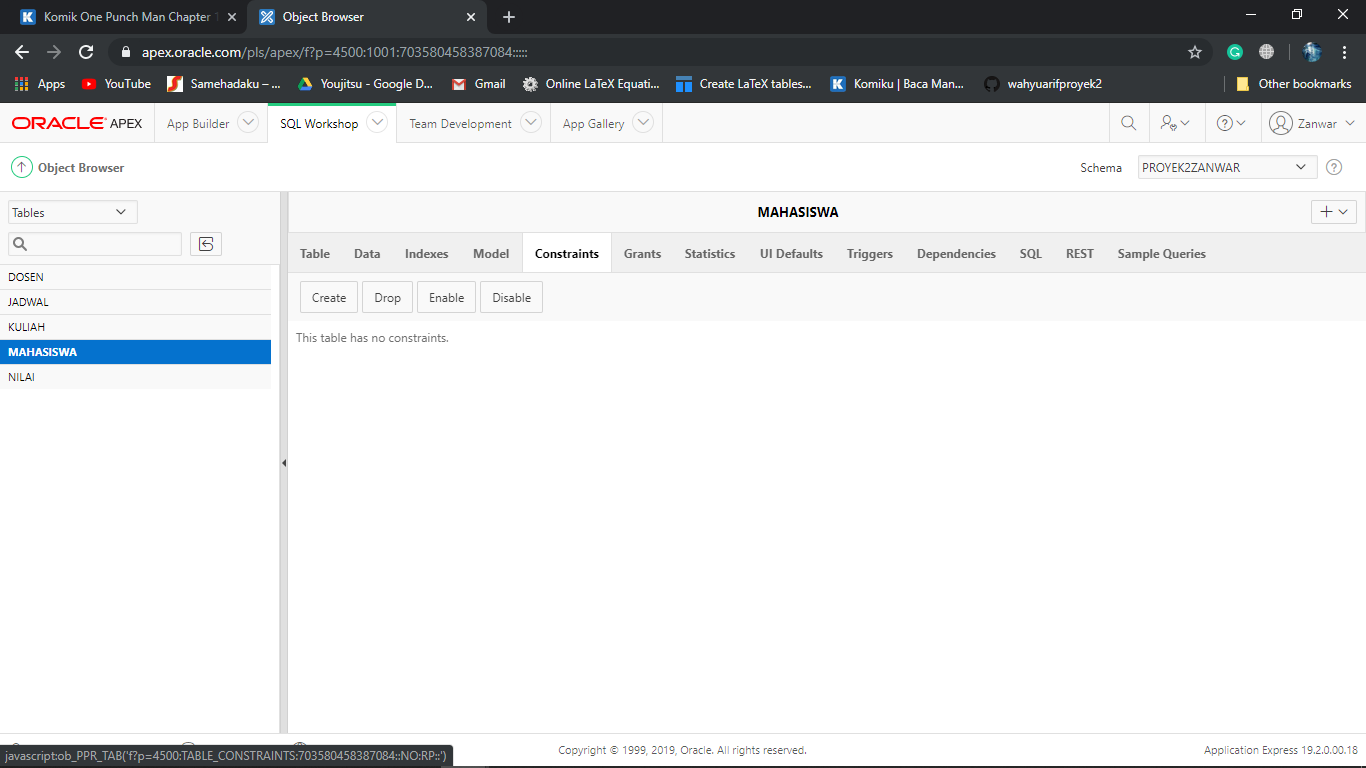
\includegraphics[scale=0.3]{figures/Screenshot(125).png}
    \caption{\textit{Add Primary Key 1.}}
    \end{center}   
    \end{figure}
    
    \begin{figure}[!htbp]
    \item[10.] Disini kita memilih attribut NIM sebagai PK karena, disini NIM attribut dengan value unique.
    \begin{center}
    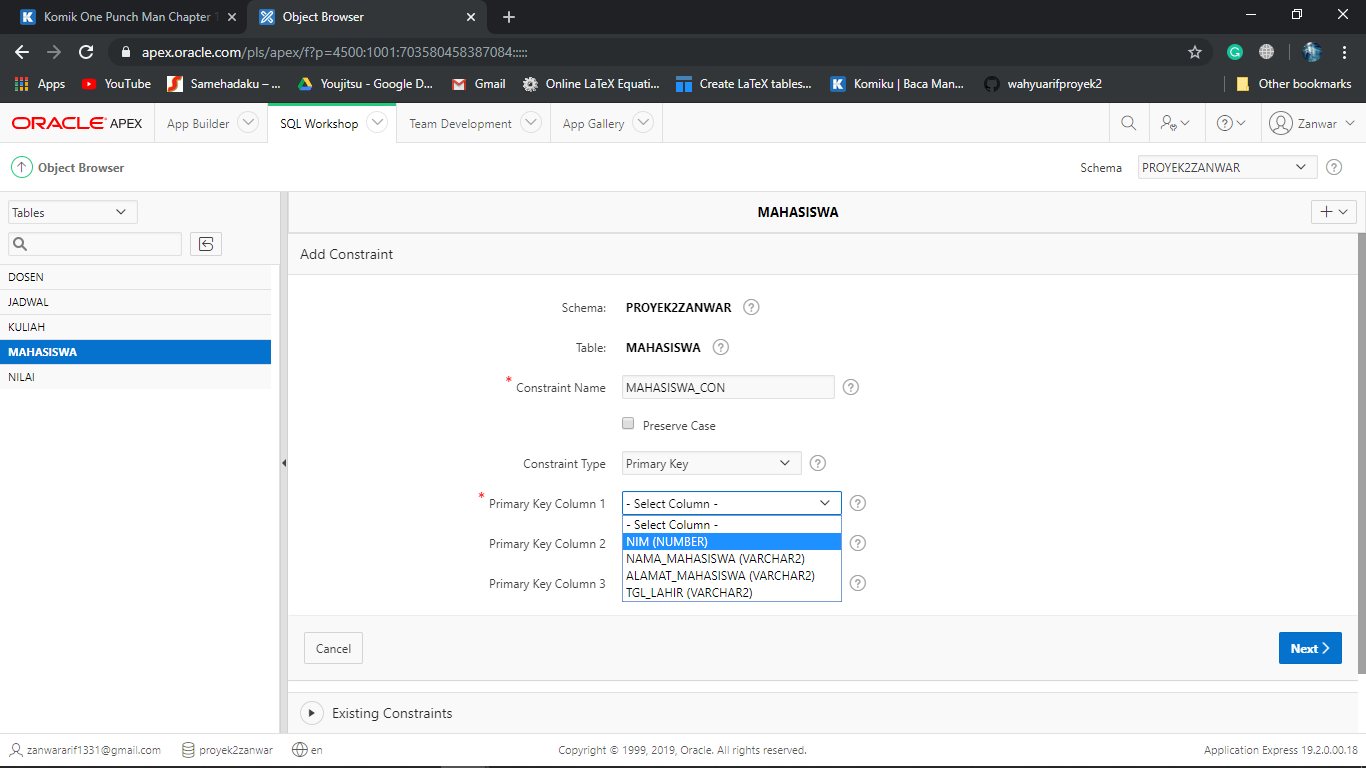
\includegraphics[scale=0.3]{figures/Screenshot(127).png}
    \caption{\textit{Add Primary Key 2.}}
    \end{center}   
    \end{figure}
    
    \begin{figure}[!htbp]
    \item[11.] Bisa dilihat yaa, kita berhasil membuat Primary key pada tabel Mahasiswa. Lakukan hal sama pada Tabel Dosen dan Kuliah.
    \begin{center}
    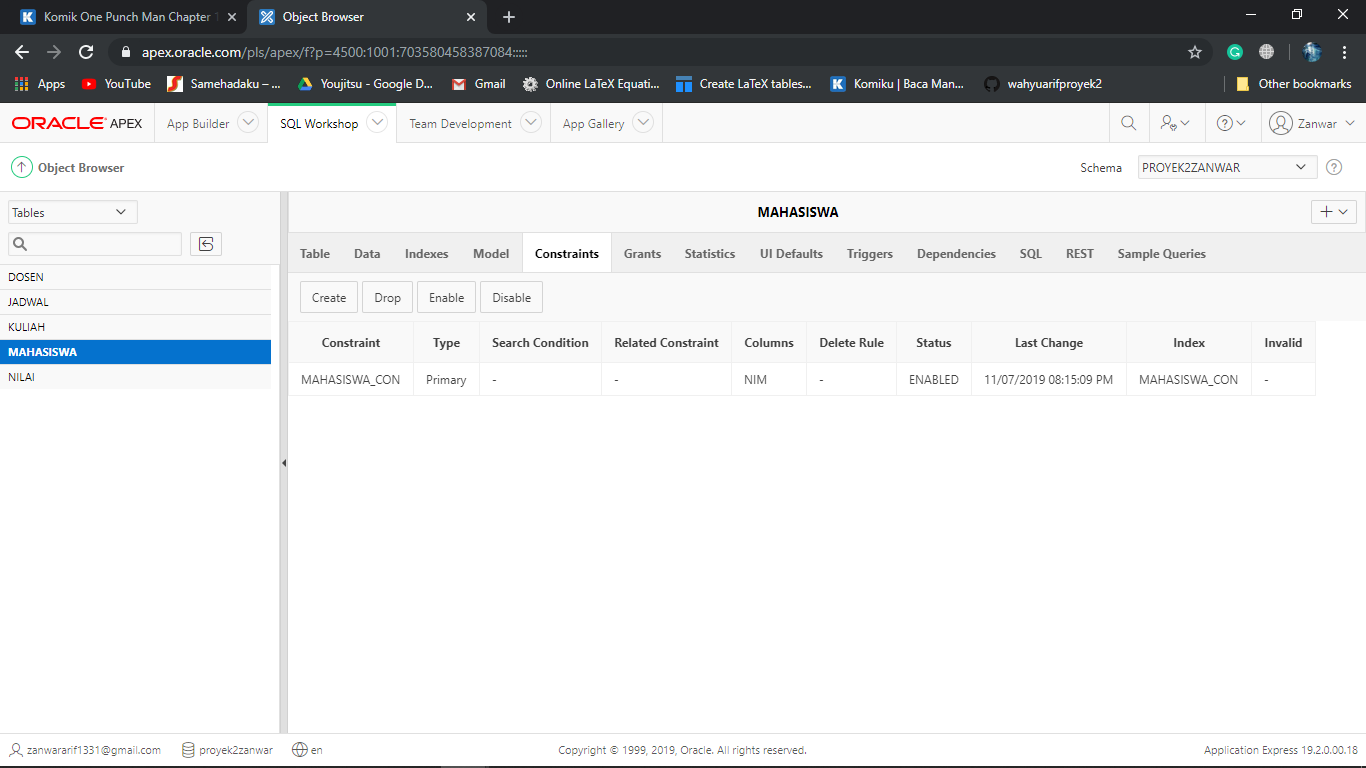
\includegraphics[scale=0.3]{figures/Screenshot(128).png}
    \caption{\textit{Add Primary Key 3.}}
    \end{center}   
    \end{figure}
    
    \begin{figure}[!htbp]
    \item[12.] Berikutnya kita akan membuat Forigen Key. Klik di constrait jugaa, bedanya saat klik create dan pilih forigen key, disini kita menentukan attribut mana yang akan dijadikan FK, dan pilih asal FK dari tabel mana dan attributnya mana.
    \begin{center}
    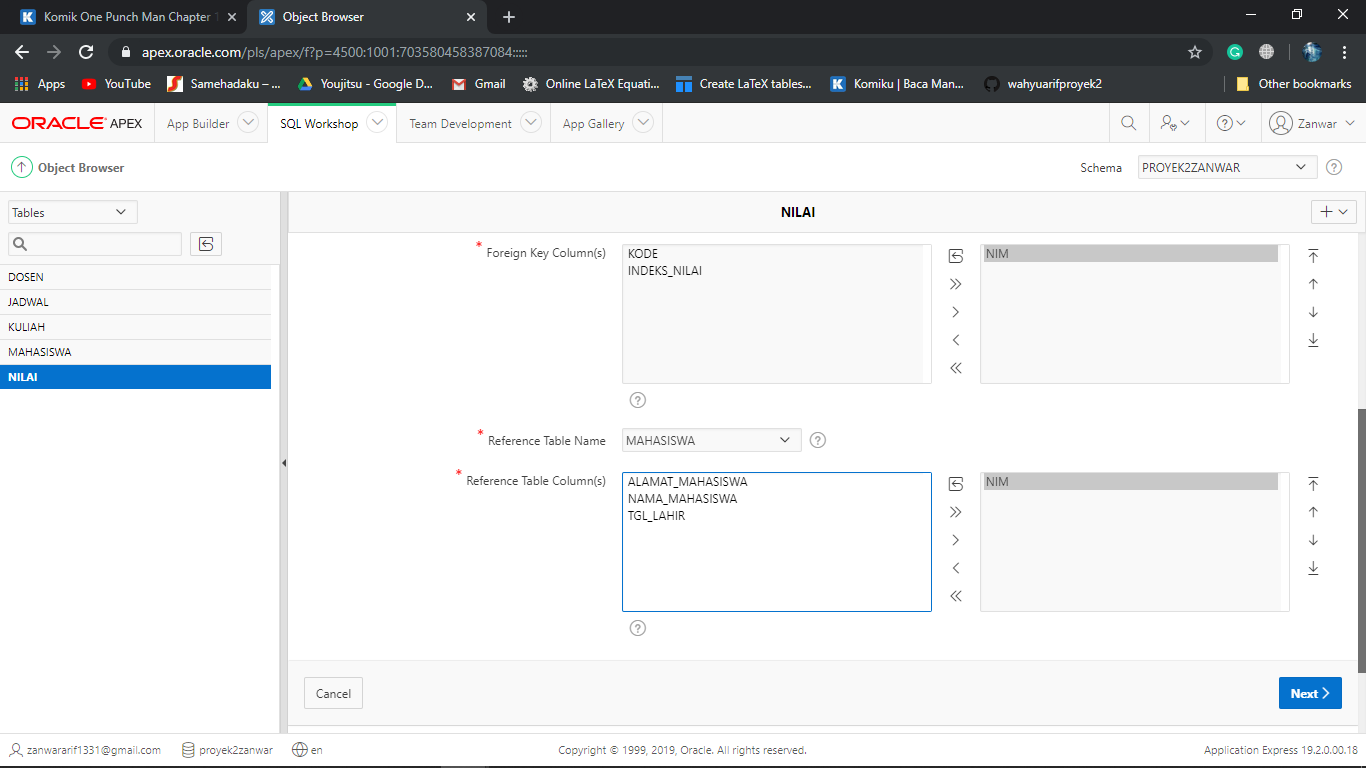
\includegraphics[scale=0.3]{figures/Screenshot(130).png}
    \caption{\textit{Add Foreign Key 1.}}
    \end{center}   
    \end{figure}
    
    \begin{figure}[!htbp]
    \item[13.] Tah, bisa dilihat kita sudah membuat 2FK pada Attribut NIM dan Kode, lakukan hal sama pada tabel jadwal.
    \begin{center}
    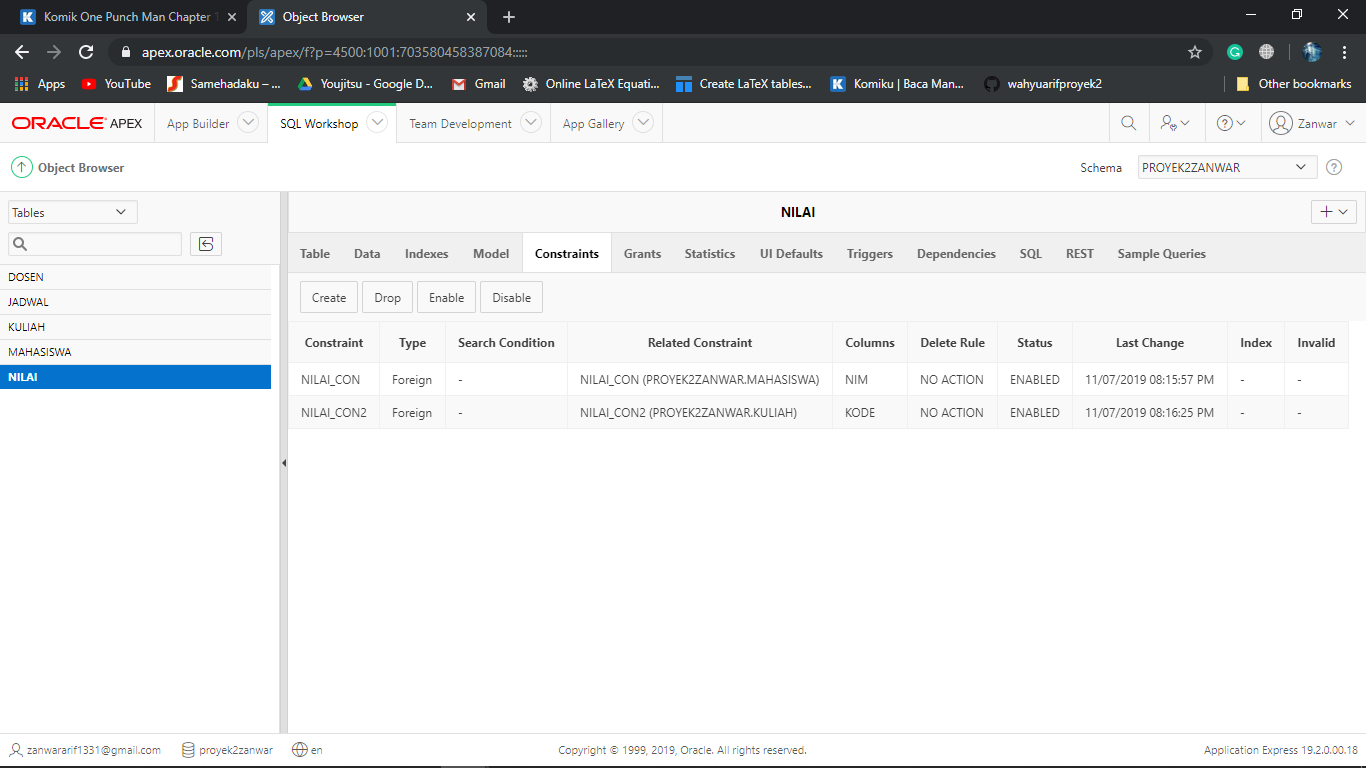
\includegraphics[scale=0.3]{figures/Screenshot(131).png}
    \caption{\textit{Add Foreign Key 2.}}
    \end{center}   
    \end{figure}
    
    \begin{figure}[!htbp]
    \item[14.] Setelah menentukan Primary key dan Forigen key pada setiap tabel, baru sekarang kita buat aplikasinya. Dengan cara klik new application.
    \begin{center}
    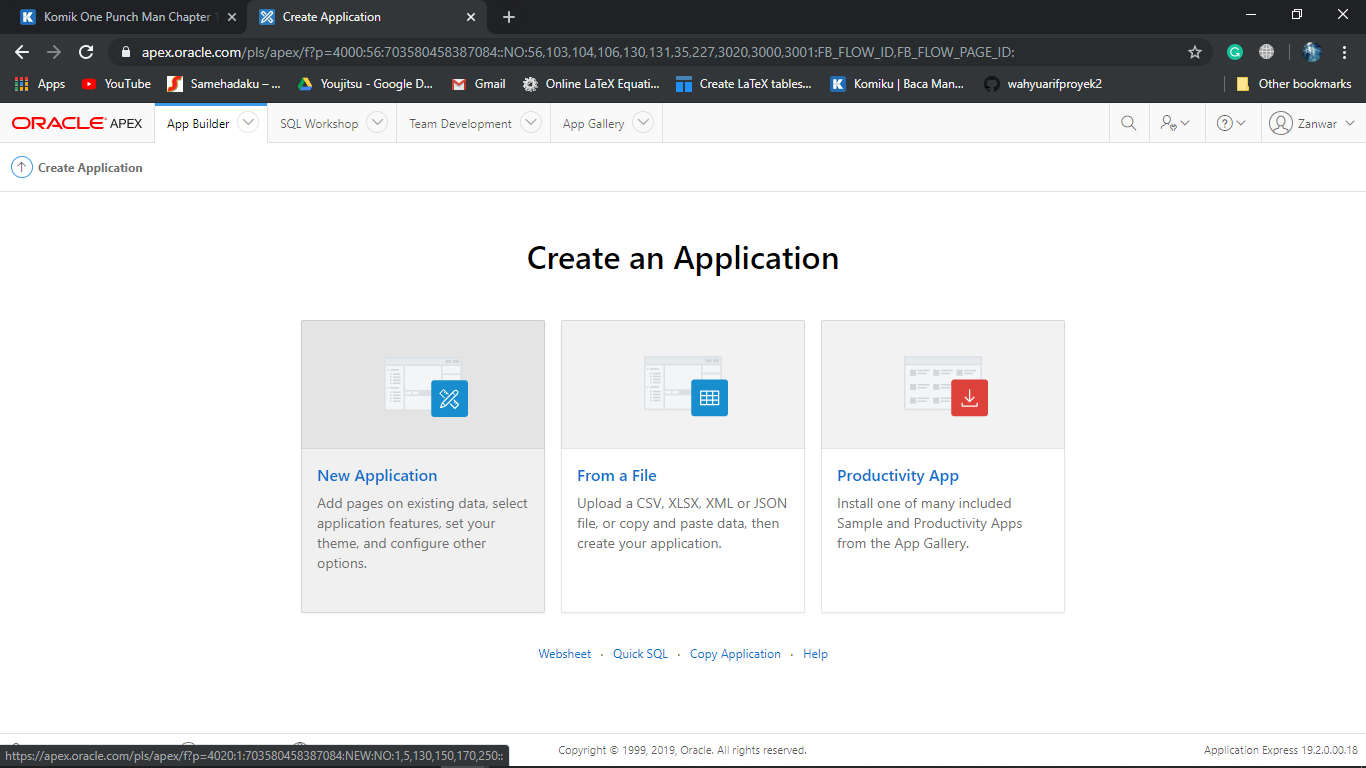
\includegraphics[scale=0.3]{figures/Screenshot(132).png}
    \caption{\textit{Create Application 1.}}
    \end{center}   
    \end{figure}
    
    \begin{figure}[!htbp]
    \item[15.] Nah disini kita Klik Add Page, lalu pilih Master Detail sesuai tugas yang diperintah oleh dosen. Tinggal tentukan Tabel yang ingin ditampilkan beserta Attributnya.
    \begin{center}
    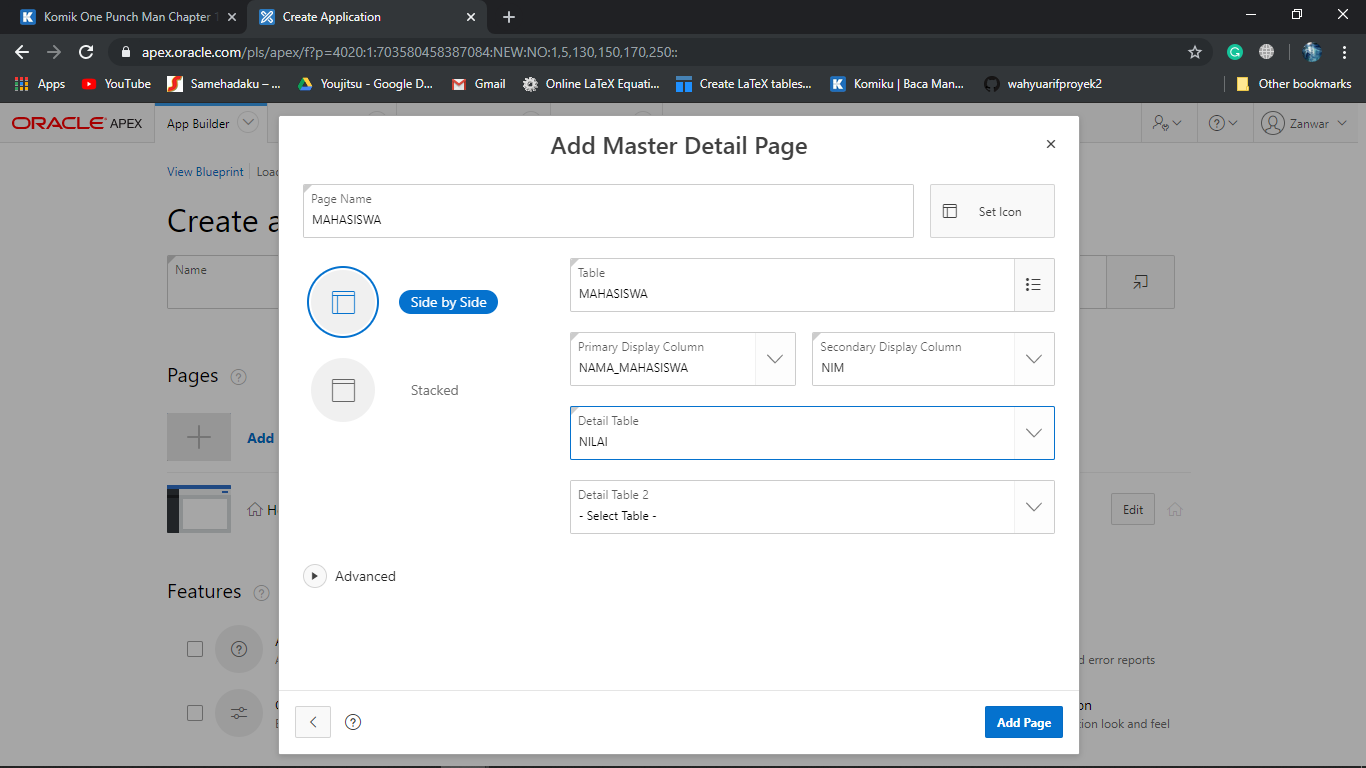
\includegraphics[scale=0.3]{figures/Screenshot(133).png}
    \caption{\textit{Add Page.}}
    \end{center}   
    \end{figure}
    
    \begin{figure}[!htbp]
    \item[16.] Jika sudah selesai membuat pagenya tinggal create application dan selesaii :)
    \begin{center}
    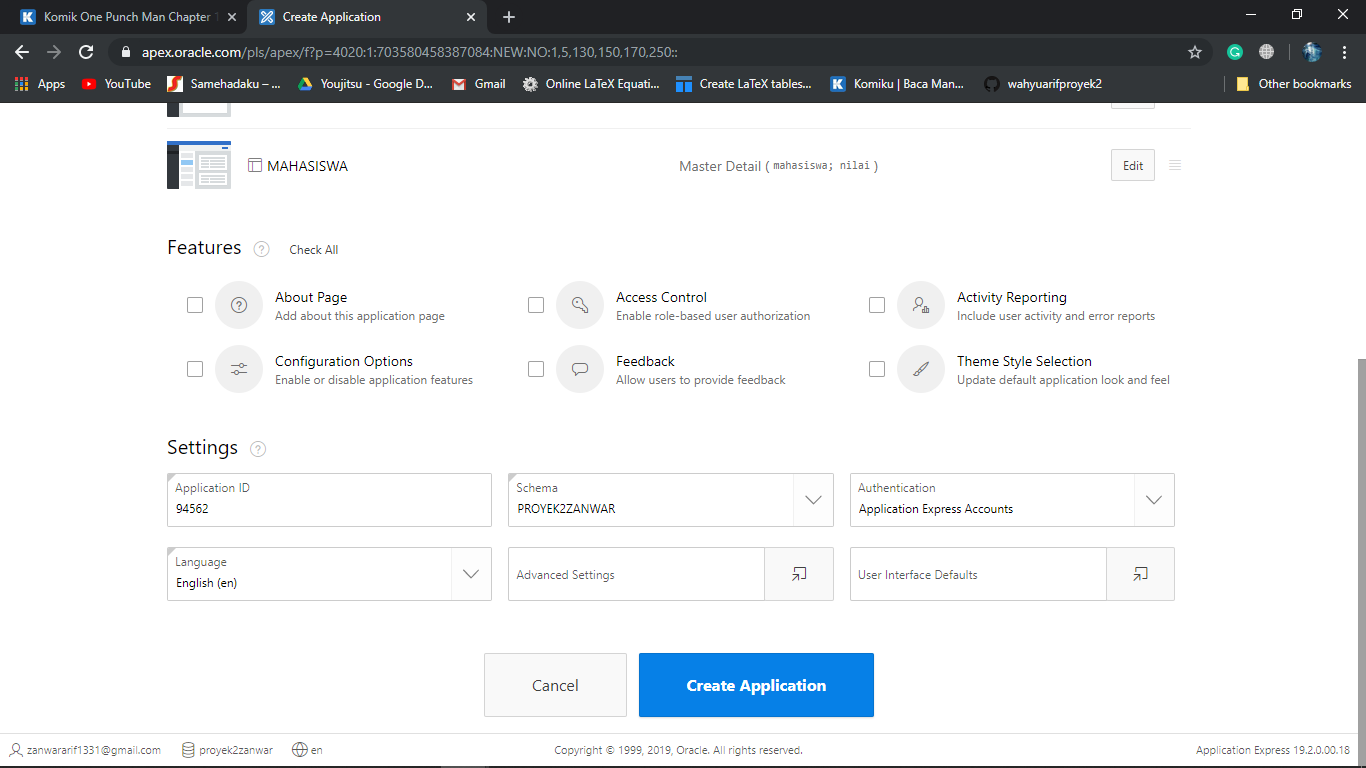
\includegraphics[scale=0.3]{figures/Screenshot(134).png}
    \caption{\textit{Create Application 2.}}
    \end{center}   
    \end{figure}
    
    \begin{figure}[!htbp]
    \item[17.] Berikut tampilan aplikasi yang sudah jadi.
    
    \par
    Bisa dicek langsung dari Link berikut:
    \par
    https://apex.oracle.com/pls/apex/f?p=67942:1:703580458387084:::::
    \par
    Dengan email: zanwararif1331@gmail.com
    \par Pass: zanwar1331
    \begin{center}
    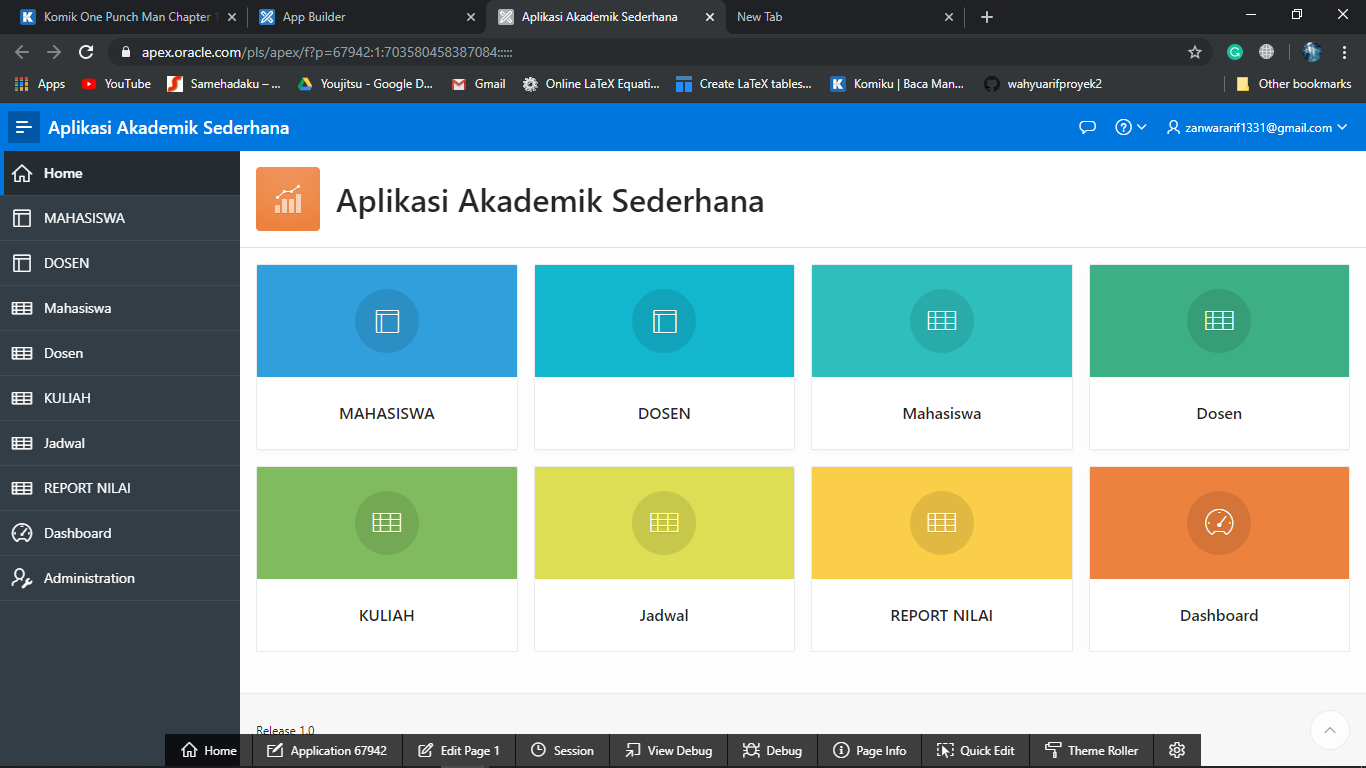
\includegraphics[scale=0.3]{figures/Screenshot(135).png}
    \caption{\textit{Aplikasi Akademik Sederhana.}}
    \end{center}   
    \end{figure}
\end{enumerate}

.